%----------------------------------------------------------------------------------------
%    PACKAGES AND THEMES
%----------------------------------------------------------------------------------------

\documentclass[aspectratio=169,xcolor=dvipsnames]{beamer}
\usetheme{SimpleDarkBlue}
\titlegraphic{
    
\includegraphics[width=3cm]{unitn-logo-1.pdf}
}
% \logo{
\includegraphics[height=1.5cm]{unitn-logo-1.pdf}}
\setbeamertemplate{footline}[frame number]{}

\usepackage{array}
\usepackage{hyperref}
\usepackage{graphicx} % Allows including images
\usepackage{booktabs} % Allows the use of \toprule, \midrule and \bottomrule in tables
\usepackage{graphicx}
\usepackage{amsmath}
\usepackage{amssymb}
\usepackage{physics}
\usepackage{braket}
\usepackage{mathpartir}
\usepackage{pdfpages}

\usepackage{glossaries}
% \makeglossaries
\newacronym{ra}{RA}{Register Assignment}
\newacronym{jair}{JAIR}{Just Another Intermediate Representation}
\newacronym{ssa}{SSA}{Static Single Assignment}
\newacronym{peo}{PEO}{Perfect Elimination Order}
\newacronym{cfg}{CFG}{Control Flow Graph}
\newacronym{bnf}{BNF}{Backus-Naur Form}
\newacronym{nasm}{NASM}{Netwise Assembler}
\newacronym{jit}{JIT}{Just-In-Time}
\newcommand{\nt}[1]{\langle\text{#1}\rangle}
\newcommand{\BareCoqSymbol}{
\includegraphics[height=0.9em]{coq.pdf}}
\newcommand{\CoqSymbol}{\raisebox{-.2ex}{\BareCoqSymbol\,}}
\newcommand{\Coqed}{{\hfill\CoqSymbol}}
\newcommand{\chordalpeosymbol}{\mathrm{Chordal}_{\gls{peo}}}
\newcommand{\chordalindsymbol}{\mathrm{Chordal}_{ind}}
\newcommand{\chordalpeo}[1]{\vdash {#1} : \chordalpeosymbol}
\newcommand{\chordalind}[1]{\vdash {#1} : \chordalindsymbol}
\newcommand{\simplicialsymbol}{\mathrm{Simplicial}}
\newcommand{\simplicial}[2]{{#2} \vdash {#1} : \simplicialsymbol}
\newcommand{\addvertex}[3]{#1 \oplus_{#2} #3}
\newcommand{\colorline}[2]{%
\begingroup
\setlength{\fboxsep}{0.5pt}%
\colorbox{#1}{#2}%
\endgroup
}

\usepackage{tikz}
\usetikzlibrary{arrows.meta, positioning, calc}
\usepackage{listings}
\lstset{
    basicstyle=\ttfamily,  % Same font as alltt
    columns=fullflexible,  % Match spacing of alltt
    keepspaces=true,       % Preserve spaces like alltt
    xleftmargin=2em,
}

\definecolor{vara}{RGB}{255,102,102}  % Red for variable a
\definecolor{varb}{RGB}{102,178,255}  % Blue for variable b
\definecolor{varc}{RGB}{102,255,102}  % Green for variable c
\definecolor{vard}{RGB}{255,178,102}  % Orange for variable d

% Colorblind-proof colors
\definecolor{StrongOrange}{RGB}{230,159,0}
\newcommand{\cbnodeA}[0]{RoyalBlue}
\newcommand{\cbnodeB}[0]{RedOrange}
\newcommand{\cbnodeC}[0]{StrongOrange}

\definecolor{myblue}{RGB}{0,0,180}
\definecolor{mygreen}{RGB}{0,120,0}
\definecolor{myred}{RGB}{180,0,0}
\definecolor{mypurple}{RGB}{120,0,120}

\lstdefinestyle{C}{
    language=C,
    mathescape=true,
    tabsize=4,
    keywordstyle=\color{myblue},              % Keywords in blue
    commentstyle=\color{mygreen!50!black},    % Comments in green
    stringstyle=\color{orange},             % Strings in orange
    showstringspaces=false,
    numbers=left,
    numberstyle=\tiny\color{gray},
    stepnumber=1,
    % frame=single,
    breaklines=true
}

\lstdefinelanguage{Rocq}{
    morekeywords=[1]{Definition, Inductive, CoInductive, Class, Instance, Fixpoint, CoFixpoint, Function, Proof, Qed, Module, Fail},
    morekeywords=[2]{forall, exists, match, with, end, if, then, else, let, in, fix, fun, intros, unfold, destruct, lia},
    morekeywords=[3]{Prop, Type, Set, True, False, nat, bool, option, list},
    sensitive=true,
    morecomment=[l]{(*},
    morecomment=[s]{(*}{*)},
    morestring=[b]",
}

\lstdefinestyle{Rocq}{
    language=Rocq,
    mathescape=true,
    keywordstyle=[1]\color{myblue},
    keywordstyle=[2]\color{mypurple},
    keywordstyle=[3]\color{myred},
    tabsize=2,
    commentstyle=\color{green!50!black}\itshape,
    stringstyle=\color{orange},
    showstringspaces=false,
    numbers=left,
    numberstyle=\tiny\color{gray},
    stepnumber=1,
    % frame=single,
    breaklines=true
}

% OCaml language with keyword groups
\lstdefinelanguage{OCaml}{
  sensitive=true,
  morecomment=[s]{(*}{*)},
  morestring=[b]",
  morekeywords=[1]{
    let, rec, in, and, val, type, module, struct, sig, class, object, method,
    inherit, virtual, functor, include, open, external, exception
  },
  morekeywords=[2]{
    if, then, else, match, with, try, when, for, to, downto, while, do, done,
    begin, end, fun, function
  },
  morekeywords=[3]{true, false},
  morekeywords=[4]{of, mutable, private, new, lazy, as, assert}
}

\lstdefinestyle{OCaml}{
    language=OCaml,
    mathescape=true,
    keywordstyle=[1]\color{myblue}\bfseries,    % Declarations
    keywordstyle=[2]\color{mypurple}\bfseries,  % Control flow
    % keywordstyle=[3]\color{orange}\bfseries,    % Constants
    keywordstyle=[4]\color{myred}\bfseries,      % Misc keywords
    tabsize=2,
    basicstyle=\ttfamily\small,
    commentstyle=\color{green!50!black}\itshape,
    stringstyle=\color{orange},
    showstringspaces=false,
    numbers=left,
    numberstyle=\tiny\color{gray},
    stepnumber=1,
    % frame=single,
    breaklines=true,
}

\lstdefinelanguage{NASM}{
  morekeywords={
    mov, add, sub, div, mul, imul, idiv, xor, and, or, inc, dec, jmp, cmp, je, jne, jl, jle, jg, jge, call, ret, push, pop, syscall
  },
  sensitive=true,
  morecomment=[n]{;}{}, % NASM uses ';' for comments
  morestring=[b]",      % Strings in double quotes
  morestring=[b]',      % Strings in single quotes
}

\lstdefinestyle{NASM}{
  language=NASM,
  keywordstyle=\color{myblue}\bfseries,
  numbers=left,
  numberstyle=\tiny\color{gray},
  stepnumber=1,
  % frame=single,
  basicstyle=\ttfamily,
  breaklines=true
}



%----------------------------------------------------------------------------------------
%    TITLE PAGE
%----------------------------------------------------------------------------------------

\title{Towards a Verified Implementation of SSA-Based Register Assignment}

\author{Giovanni Maria Zanchetta}
\institute
{
    Advisor: Prof. Marco Patrignani \\
    Co-Advisor: Matthis Kruse \\
}
\date{September 2025}

%----------------------------------------------------------------------------------------
%    PRESENTATION SLIDES
%----------------------------------------------------------------------------------------

\begin{document}

\begin{frame}
    % Print the title page as the first slide
    \titlepage
\end{frame}

\begin{frame}{Overview}
    % Throughout your presentation, if you choose to use \section{} and \subsection{} commands, these will automatically be printed on this slide as an overview of your presentation
    \tableofcontents
\end{frame}

\section{Context}
\begin{frame}{Register Assignment}
% Errors

\centering
\begin{minipage}{0.58\linewidth}
    \begin{tabular}{|c|p{3cm}|c|c|c|c|c|}
    \hline
    \textbf{Line} & \textbf{Code} & \textbf{a} & \textbf{b} & \textbf{c} & \textbf{d} & \textbf{e} \\
    \hline
    1 & \lstinline[style=C]|int a = $\dots$;| & & & & & \\
    \hline
    2 & \lstinline[style=C]|int b = $\dots$;| & $\bullet$ & & & & \\
    \hline
    3 & \lstinline[style=C]|int c = a + b;| & $\bullet$ & $\bullet$ & & & \\
    \hline
    4 & \lstinline[style=C]|int d = a + c;| & $\bullet$ & $\bullet$ & $\bullet$ & & \\
    \hline
    5 & \lstinline[style=C]|int e = b + d;| & & $\bullet$ & & $\bullet$ & \\
    \hline
    6 & \lstinline[style=C]|return e;| & & & & & $\bullet$ \\
    \hline
    \end{tabular}
\end{minipage}
\hfill
\begin{minipage}{0.38\linewidth}
    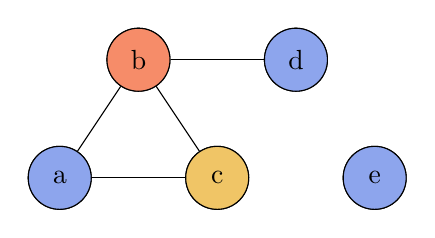
\begin{tikzpicture}[scale=1, every node/.style={circle, draw, minimum size=8mm}]
    \node<1> (a) at (0,0)      {a};
    \node<1> (b) at (1,1.5)    {b};
    \node<1> (c) at (2,0)      {c};
    \node<1> (d) at (3,1.5)    {d};
    \node<1> (e) at (4,0)    {e};
    \node<2>[fill=\cbnodeA!60] (a) at (0,0)      {a};
    \node<2>[fill=\cbnodeB!60] (b) at (1,1.5)    {b};
    \node<2>[fill=\cbnodeC!60] (c) at (2,0)      {c};
    \node<2>[fill=\cbnodeA!60] (d) at (3,1.5)    {d};
    \node<2>[fill=\cbnodeA!60] (e) at (4,0)    {e};

    \draw<1, 2>(a) -- (b);
    \draw<1, 2>(a) -- (c);
    \draw<1, 2>(b) -- (c);
    \draw<1, 2>(b) -- (d);
  \end{tikzpicture}
\end{minipage}

\hfill

\begin{definition}[Interference Graph]
    Graph $G = (V, E)$ such that \begin{itemize}
        \item $V$ is the set of variables;
        \item $E$ is the set of edges such that $\{ u, v \} \in E$, iff variables $u$ and $v$ interfere;
    \end{itemize}
\end{definition}
\end{frame}

\begin{frame}{Graph Coloring-Based Register Assignment}
% Errors

% B0:
% r0 <- 5
% if r0 < 10 then B1 else B2
%
% B1:
% r1 <- r0
%
% B2:
% r2 <- r0 + 2
%
% B3:
% r3 <- phi r1 r2
% r4 <- r0 + r3

\begin{definition}[Static Single Assignment (SSA)]
    A program is in SSA form iff:
    \begin{itemize}
        \item Every variable is defined \textit{exactly} once;
        \item For every variable, its definition comes before its usages.
    \end{itemize}
\end{definition}

\vfill

\begin{minipage}{0.48\linewidth}
\centering
\begin{tikzpicture}[
    node distance=10mm,
    every node/.style={draw, align=left, inner sep=4pt},
    >={Stealth}
]
\node (entry) at (0, 0) [draw, label=left:$B_0$] {
    $\textcolor<8->{\cbnodeA}{r_0} \leftarrow 5$ \\
    $\textcolor<9->{\cbnodeB}{r_1} \leftarrow 10$ \\
    if $\textcolor<8->{\cbnodeA}{r_0} < \textcolor<9->{\cbnodeB}{r_1}$
};
\node (b1) at (-1.7, -1.4) [draw, label=left:$B_1$] {
    $\textcolor<10->{\cbnodeC}{r_2} \leftarrow \textcolor<8->{\cbnodeA}{r_0} + 1$
};
\node (b2) at (1.7, -1.4) [draw, label=right:$B_2$] {
    $\textcolor<11->{\cbnodeC}{r_3} \leftarrow \textcolor<8->{\cbnodeA}{r_0} + 2$
};
\node (end) at (0, -2.85) [draw, label=left:$B_3$] {
    $\textcolor<12->{\cbnodeB}{r_4} \leftarrow \phi(\textcolor<10->{\cbnodeC}{r_2}, \textcolor<11->{\cbnodeC}{r_3})$ \\
    $\textcolor<13->{\cbnodeA}{r_5} \leftarrow \textcolor<8->{\cbnodeA}{r_0} + \textcolor<9->{\cbnodeB}{r_1}$ \\
    ret $\textcolor<12->{\cbnodeB}{r_4}$
};
\draw[->] (entry) -- (b1);
\draw[->] (entry) -- (b2);
\draw[->] (b1) -- (end);
\draw[->] (b2) -- (end);
\end{tikzpicture}

\end{minipage}
\hfill
\begin{minipage}{0.48\linewidth}
\begin{center}
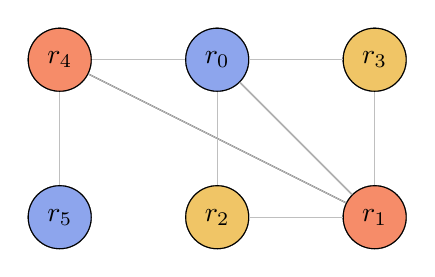
\begin{tikzpicture}[scale=1, every node/.style={circle, draw, minimum size=8mm}]
\node<-6> (r0) at (0,0) {$r_0$};
\node<-5> (r1) at (2,-2) {$r_1$};
\node<-3> (r2) at (0,-2) {$r_2$};
\node<-4> (r3) at (2,0) {$r_3$};
\node<-2> (r4) at (-2,0) {$r_4$};
\node<-1> (r5) at (-2,-2) {$r_5$};

\node<7-7>[draw=lightgray, text=lightgray] (r0) at (0,0) {$r_0$};
\node<6-8>[draw=lightgray, text=lightgray] (r1) at (2,-2) {$r_1$};
\node<4-10>[draw=lightgray, text=lightgray] (r2) at (0,-2) {$r_2$};
\node<5-9>[draw=lightgray, text=lightgray] (r3) at (2,0) {$r_3$};
\node<3-11>[draw=lightgray, text=lightgray] (r4) at (-2,0) {$r_4$};
\node<2-12>[draw=lightgray, text=lightgray] (r5) at (-2,-2) {$r_5$};

\node<8->[fill=\cbnodeA!60] (r0) at (0,0) {$r_0$};
\node<9->[fill=\cbnodeB!60] (r1) at (2,-2) {$r_1$};
\node<11->[fill=\cbnodeC!60] (r2) at (0,-2) {$r_2$};
\node<10->[fill=\cbnodeC!60] (r3) at (2,0) {$r_3$};
\node<12->[fill=\cbnodeB!60] (r4) at (-2,0) {$r_4$};
\node<13->[fill=\cbnodeA!60] (r5) at (-2,-2) {$r_5$};

\draw<-5,9-> (r0) -- (r1);
\draw<-3,11-> (r0) -- (r2);
\draw<-4,10-> (r0) -- (r3);
\draw<-2,12-> (r0) -- (r4);
\draw<-3,11-> (r1) -- (r2);
\draw<-4,10-> (r1) -- (r3);
\draw<-2,12-> (r1) -- (r4);
\draw<-1,13-> (r4) -- (r5);
\draw<6-8>[draw=lightgray] (r0) -- (r1);
\draw<4-10>[draw=lightgray] (r0) -- (r2);
\draw<5-9>[draw=lightgray] (r0) -- (r3);
\draw<3-11>[draw=lightgray] (r0) -- (r4);
\draw<4-10>[draw=lightgray] (r1) -- (r2);
\draw<5-9>[draw=lightgray] (r1) -- (r3);
\draw<3-11>[draw=lightgray] (r1) -- (r4);
\draw<2-12>[draw=lightgray] (r4) -- (r5);
\end{tikzpicture}
\end{center}

\centering
\only<1>    {PEO:}
\only<2>    {PEO: $r_5$}
\only<3>    {PEO: $r_5, r_4$}
\only<4>    {PEO: $r_5, r_4, r_2$}
\only<5>    {PEO: $r_5, r_4, r_2, r_3$}
\only<6>    {PEO: $r_5, r_4, r_2, r_3, r_1$}
\only<7>    {PEO: $r_5, r_4, r_2, r_3, r_1, r_0$}
\only<8>    {PEO: $r_5, r_4, r_2, r_3, r_1 \textcolor{lightgray}{, r_0}$}
\only<9>    {PEO: $r_5, r_4, r_2, r_3 \textcolor{lightgray}{, r_1, r_0}$}
\only<10>   {PEO: $r_5, r_4, r_2 \textcolor{lightgray}{, r_3, r_1, r_0}$}
\only<11>   {PEO: $r_5, r_4 \textcolor{lightgray}{, r_2, r_3, r_1, r_0}$}
\only<12>   {PEO: $r_5 \textcolor{lightgray}{, r_4, r_2, r_3, r_1, r_0}$}
\only<13>   {PEO: $\textcolor{lightgray}{r_5, r_4, r_2, r_3, r_1, r_0}$}

\end{minipage}
\end{frame}

\begin{frame}{Single Static Assignment}
% Errors

\begin{definition}[Single Static Assignment (SSA)]
    A program is in SSA form iff:
    \begin{itemize}
        \item Every variable is defined \textit{exactly} once;
        \item For every variable, its definition comes before its usages;
    \end{itemize}
\end{definition}

\only<1>{
\centering
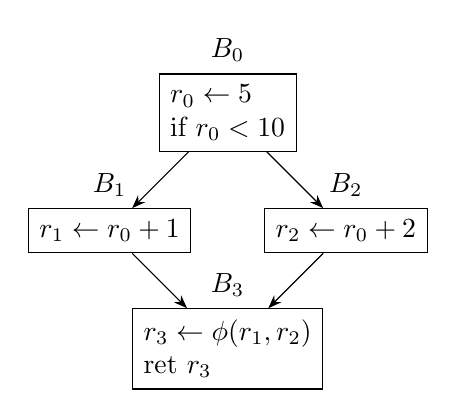
\begin{tikzpicture}[
    node distance=10mm,
    every node/.style={draw, align=left, inner sep=4pt},
    >={Stealth}
]
\node (entry)   at (0, 0)       [draw, label=above:$B_0$]   {$r_0 \leftarrow 5$ \\ if $r_0 < 10$};
\node (b1)      at (-1.5, -1.5) [draw, label=above:$B_1$]   {$r_1 \leftarrow r_0 + 1$};
\node (b2)      at (1.5, -1.5)  [draw, label=above:$B_2$]   {$r_2 \leftarrow r_0 + 2$};
\node (end)     at (0, -3)      [draw, label=above:$B_3$]   {$r_3 \leftarrow \phi(r_1, r_2)$ \\ ret $r_3$};

\draw[->] (entry) -- (b1);
\draw[->] (entry) -- (b2);
\draw[->] (b1) -- (end);
\draw[->] (b2) -- (end);
\end{tikzpicture}
}
\end{frame}

\begin{frame}{Chordality Theorem}
% Errors

\only<1>{
\begin{minipage}{0.55\linewidth}
\centering
\[
\renewcommand{\arraystretch}{1}
\begin{array}{l}
\text{Block (Normal 3) } [ \\
\quad r(4) \leftarrow \phi[(0, \ \text{Normal 1}); \ (2, \ \text{Normal 2})]; \\
\quad r(5) \leftarrow \phi[(1, \ \text{Normal 1}); \ (3, \ \text{Normal 2})] \\
] \ [ \\
\quad r(6) \leftarrow r(4) \times r(5); \\
\quad r(7) \leftarrow r(6) + i(1) \\
] \ ( \\
\quad \text{if } r(7) \leq i(100) \text{ then } \dots \text{ else } \dots \\
)
\end{array}
\]
\end{minipage}
\hfill
\begin{minipage}{0.40\linewidth}
\centering
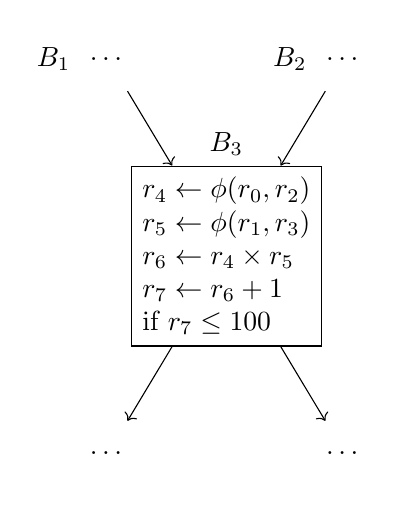
\begin{tikzpicture}
\node (b1) at (-1.5, 0) [minimum height=0.8cm, label=left:$B_1$] {$\dots$};
\node (b2) at (1.5, 0) [minimum height=0.8cm, label=left:$B_2$] {$\dots$};
\node (b3) at (0, -2.5) [draw, align=left, inner sep=4pt, label=above:$B_3$] {$r_4 \leftarrow \phi(r_0, r_2)$ \\ $r_5 \leftarrow \phi(r_1, r_3)$ \\ $r_6 \leftarrow r_4 \times r_5$ \\ $r_7 \leftarrow r_6 + 1$ \\ if $r_7 \leq 100$};
\node (b4) at (-1.5, -5) [minimum height=0.8cm] {$\dots$};
\node (b5) at (1.5, -5) [minimum height=0.8cm] {$\dots$};

\draw[->] (b1) -- (b3);
\draw[->] (b2) -- (b3);
\draw[->] (b3) -- (b4);
\draw[->] (b3) -- (b5);
\end{tikzpicture}
\end{minipage}
}

\only<2>{
\centering
\begin{minipage}{0.55\linewidth}
\centering
\[
\renewcommand{\arraystretch}{1}
\begin{array}{l}
\text{Block (Normal 3) } [ \\
\quad r(\texttt{rdx}) \leftarrow \phi[(\texttt{rdx}, \ \text{Normal 1}); \ (\texttt{rdx}, \ \text{Normal 2})]; \\
\quad r(\texttt{rbx}) \leftarrow \phi[(\texttt{rbx}, \ \text{Normal 1}); \ (\texttt{rbx}, \ \text{Normal 2})]; \\
] \ [ \\
\quad r(\texttt{rbx}) \leftarrow r(\texttt{rdx}) \times r(\texttt{rbx}); \\
\quad r(\texttt{rbx}) \leftarrow r(\texttt{rbx}) + i(1); \\
] \ ( \\
\quad \text{if } r(\texttt{rbx}) \leq i(100) \text{ then } \dots \text{ else } \dots \\
)
\end{array}
\]
\end{minipage}
\hfill
\begin{minipage}{0.40\linewidth}
\centering
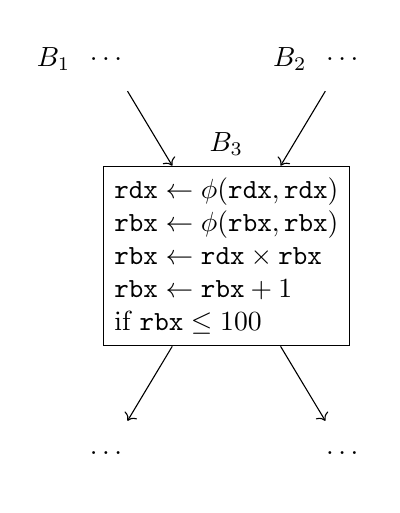
\begin{tikzpicture}
\node (b1) at (-1.5, 0) [minimum height=0.8cm, label=left:$B_1$] {$\dots$};
\node (b2) at (1.5, 0) [minimum height=0.8cm, label=left:$B_2$] {$\dots$};
\node (b3) at (0, -2.5) [draw, align=left, inner sep=4pt, label=above:$B_3$] {$\texttt{rdx} \leftarrow \phi(\texttt{rdx}, \texttt{rdx})$ \\ $\texttt{rbx} \leftarrow \phi(\texttt{rbx}, \texttt{rbx})$ \\ $\texttt{rbx} \leftarrow \texttt{rdx} \times \texttt{rbx}$ \\ $\texttt{rbx} \leftarrow \texttt{rbx} + 1$ \\ if $\texttt{rbx} \leq 100$};
\node (b4) at (-1.5, -5) [minimum height=0.8cm] {$\dots$};
\node (b5) at (1.5, -5) [minimum height=0.8cm] {$\dots$};

\draw[->] (b1) -- (b3);
\draw[->] (b2) -- (b3);
\draw[->] (b3) -- (b4);
\draw[->] (b3) -- (b5);
\end{tikzpicture}
\end{minipage}
}

% \only<1>{
% \begin{align*}
% \nt{label} &::= \text{Normal} \ \mathbb N \mid \text{Point1} \ \mathbb N \mid \text{Point2} \ \mathbb N
% \\
% \nt{value} &::= i( \mathbb Z ) \mid r( \nt{register} ) \mid p( \mathbb N )
% \\
% \nt{expression} &::= \nt{value} \\
% &\mid \text{load} \ \nt{value} \\
% &\mid r( \nt{register} ) \makebox[1em]{+} \nt{value} \\
% &\mid r( \nt{register} ) \makebox[1em]{-} \nt{value} \\
% &\mid r( \nt{register} ) \makebox[1em]{*} \nt{value} \\
% &\mid r( \nt{register} ) \makebox[1em]{/} \nt{value}
% \\
% \nt{instruction} &::= r( \nt{register} ) \leftarrow \nt{expression} \\
% &\mid \text{store} \ r( \nt{register} ) \ r( \nt{register} )
% \\
% \nt{instructions} &::= \nt{instruction} ; \ \nt{instructions} \mid \nt{instruction}
% \\
% \nt{instructions-or-nil} &::= [ \nt{instructions} ] \mid []
% \end{align*}
% }

% \only<2>{
% \begin{align*}
% \nt{phi-arguments} &::= ( \nt{register} , \ \nt{label} ) ; \ \nt{phi-arguments} \\
% &\mid (\nt{register} , \ \nt{label})
% \\
% \nt{phi} &::= r( \nt{register} ) \leftarrow \phi \ \nt{phi-arguments-or-nil}
% \\
% \nt{phis} &::= \nt{phi} ; \ \nt{phis}
% \\
% \nt{phis-or-nil} &::= [ \nt{phis} ] \mid []
% \end{align*}
% }

% \only<3>{
% \begin{align*}
% \nt{condition} &::= r(\nt{register}) = \nt{val} \\
% &\mid r(\nt{register}) \neq \nt{val} \\
% &\mid r(\nt{register}) < \nt{val} \\
% &\mid r(\nt{register}) \leq \nt{val} \\
% &\mid r(\nt{register}) > \nt{val} \\
% &\mid r(\nt{register}) \geq \nt{val}
% \\
% \nt{jump-instruction} &::= \text{if} \ \nt{condition} \ \text{then} \ \nt{block} \ \text{else} \ \nt{block} \\
% &\mid \text{jump} \ \nt{block} \\
% &\mid \text{ret} \ r( \nt{register} )
% \\
% \nt{block} &::= \text{Block} \ ( \nt{label} ) \ \nt{phis-or-nil} \ \nt{instructions-or-nil} \ ( \nt{jump-instruction} )
% \end{align*}
% }
\end{frame}

\begin{frame}{Register Allocation Algorithm}
% Errors

\begin{lstlisting}[style=Rocq]
Inductive vm : Type :=
  | Vm : (reg -> word) -> list word -> vm.

Definition get_reg (m : vm) (r : reg) : word :=
  (* ... *)

Definition set_reg (m : vm) (r : reg) (c : word) : vm :=
  (* ... *)

Definition get_word (m : vm) (i : nat) : word :=
  (* ... *)

Definition set_word (m : vm) (i : nat) (c : word) : vm :=
  (* ... *)
\end{lstlisting}

% \only<1>{
% \begin{align*}
% \nt{label} &::= \text{Normal} \ \mathbb N \mid \text{Point1} \ \mathbb N \mid \text{Point2} \ \mathbb N
% \\
% \nt{value} &::= i( \mathbb Z ) \mid r( \nt{register} ) \mid p( \mathbb N )
% \\
% \nt{expression} &::= \nt{value} \\
% &\mid \text{load} \ \nt{value} \\
% &\mid r( \nt{register} ) \makebox[1em]{+} \nt{value} \\
% &\mid r( \nt{register} ) \makebox[1em]{-} \nt{value} \\
% &\mid r( \nt{register} ) \makebox[1em]{*} \nt{value} \\
% &\mid r( \nt{register} ) \makebox[1em]{/} \nt{value}
% \\
% \nt{instruction} &::= r( \nt{register} ) \leftarrow \nt{expression} \\
% &\mid \text{store} \ r( \nt{register} ) \ r( \nt{register} )
% \\
% \nt{instructions} &::= \nt{instruction} ; \ \nt{instructions} \mid \nt{instruction}
% \\
% \nt{instructions-or-nil} &::= [ \nt{instructions} ] \mid []
% \end{align*}
% }

% \only<2>{
% \begin{align*}
% \nt{phi-arguments} &::= ( \nt{register} , \ \nt{label} ) ; \ \nt{phi-arguments} \\
% &\mid (\nt{register} , \ \nt{label})
% \\
% \nt{phi} &::= r( \nt{register} ) \leftarrow \phi \ \nt{phi-arguments-or-nil}
% \\
% \nt{phis} &::= \nt{phi} ; \ \nt{phis}
% \\
% \nt{phis-or-nil} &::= [ \nt{phis} ] \mid []
% \end{align*}
% }

% \only<3>{
% \begin{align*}
% \nt{condition} &::= r(\nt{register}) = \nt{val} \\
% &\mid r(\nt{register}) \neq \nt{val} \\
% &\mid r(\nt{register}) < \nt{val} \\
% &\mid r(\nt{register}) \leq \nt{val} \\
% &\mid r(\nt{register}) > \nt{val} \\
% &\mid r(\nt{register}) \geq \nt{val}
% \\
% \nt{jump-instruction} &::= \text{if} \ \nt{condition} \ \text{then} \ \nt{block} \ \text{else} \ \nt{block} \\
% &\mid \text{jump} \ \nt{block} \\
% &\mid \text{ret} \ r( \nt{register} )
% \\
% \nt{block} &::= \text{Block} \ ( \nt{label} ) \ \nt{phis-or-nil} \ \nt{instructions-or-nil} \ ( \nt{jump-instruction} )
% \end{align*}
% }
\end{frame}

\section{Just Another Intermediate Representation (JAIR)}

\begin{frame}{The JAIR Syntax}
% Errors

\begin{overlayarea}{\textwidth}{8cm}
\begin{onlyenv}
\begin{lstlisting}[style=Rocq]
Definition is_simplicialb (G : IFG) (r : reg) : bool :=
  r $\in$ G.V $\land$ is_cliqueb G[v].
\end{lstlisting}
\end{onlyenv}

\begin{onlyenv}<2,3,4>
\begin{lstlisting}[style=Rocq]
Definition find_next (G : IFG) : option reg :=
  find (is_simplicialb G) G.V.
\end{lstlisting}
\end{onlyenv}

\begin{onlyenv}<3,4>
\begin{lstlisting}[style=Rocq]
Definition eliminate_step (G : IFG) : option (reg * IFG) :=
  let* u = find_next G in Some (u, G - u).
\end{lstlisting}
\end{onlyenv}

\begin{onlyenv}<4>
\begin{lstlisting}[style=Rocq]
Function eliminate (G : IFG) {measure |G.V|} : list reg :=
  match eliminate_step G with
  | Some (u, G') => in u :: (eliminate G')
  | None => []
  end.
\end{lstlisting}
\end{onlyenv}
\end{overlayarea}
\end{frame}

\section{Implementation of \texttt{eliminate}}

\begin{frame}{Implementation of \texttt{eliminate}}
% Errors

\only<1>{
\centering

$\boxed{\simplicial{u}{G}}$ In the context of graph $G$, node $u$ is simplicial.

\vfill

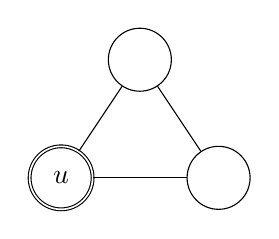
\begin{tikzpicture}
    \node[circle, double, draw, minimum size=8mm] (a) at (0,0) {$u$};
    \node[circle, draw, minimum size=8mm] (b) at (1,1.5) {};
    \node[circle, draw, minimum size=8mm] (c) at (2,0) {};

    \draw (a) -- (b);
    \draw (a) -- (c);
    \draw (b) -- (c);
\end{tikzpicture}
}

\only<2>{
\[
\inferrule*[Right=SimplicialSingleton]
    {\textcolor{red}{u} \not \in V}
    {\simplicial{\textcolor{red}{u}}{G + \textcolor{red}{u}}}
\]

\vfill

\centering
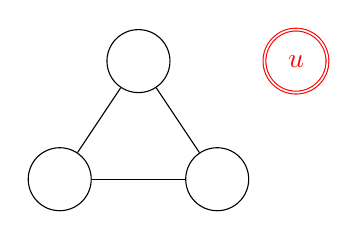
\begin{tikzpicture}
    \node[circle, draw, minimum size=8mm] (a) at (0,0) {};
    \node[circle, draw, minimum size=8mm] (b) at (1,1.5) {};
    \node[circle, draw, minimum size=8mm] (c) at (2,0) {};
    \node[circle, double, draw=red, text=red, minimum size=8mm] at (3,1.5) {$u$};

    \draw (a) -- (b);
    \draw (a) -- (c);
    \draw (b) -- (c);
\end{tikzpicture}
}

\only<3>{
\[
\inferrule*[Right=SimplicialNode]
    {\simplicial{u}{G}}
    {\simplicial{u}{G + \textcolor{red}{v}}}
\]

\vfill

\centering
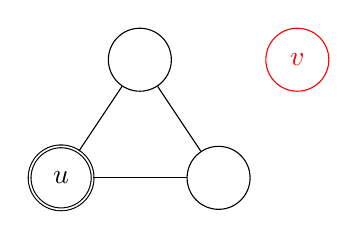
\begin{tikzpicture}
    \node[circle, double, draw, minimum size=8mm] (a) at (0,0) {$u$};
    \node[circle, draw, minimum size=8mm] (b) at (1,1.5) {};
    \node[circle, draw, minimum size=8mm] (c) at (2,0) {};
    \node[circle, draw=red, text=red, minimum size=8mm] at (3,1.5) {$v$};

    \draw (a) -- (b);
    \draw (a) -- (c);
    \draw (b) -- (c);
\end{tikzpicture}
}

\only<4>{
\[
\inferrule*[Right=SimplicialEdge]
    {\simplicial{u}{G} \\ u \neq \textcolor{red}{v} \\ u \neq \textcolor{red}{w}}
    {\simplicial{u}{G + \{ \textcolor{red}{v}, \textcolor{red}{w} \}}}
\]

\vfill

\centering
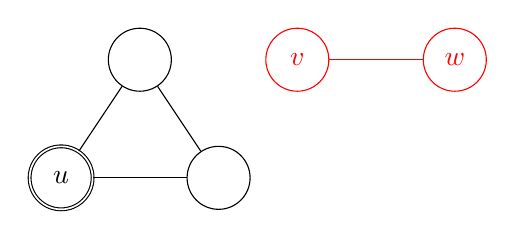
\begin{tikzpicture}
    \node[circle, double, draw, minimum size=8mm] (a) at (0,0) {$u$};
    \node[circle, draw, minimum size=8mm] (b) at (1,1.5) {};
    \node[circle, draw, minimum size=8mm] (c) at (2,0) {};
    \node[circle, draw=red, text=red, minimum size=8mm] (v) at (3,1.5) {$v$};
    \node[circle, draw=red, text=red, minimum size=8mm] (w) at (5,1.5) {$w$};

    \draw (a) -- (b);
    \draw (a) -- (c);
    \draw (b) -- (c);
    \draw[draw=red] (v) -- (w);
\end{tikzpicture}
}

\only<5>{
\[
\inferrule*[Right=SimplicialNeighbor]
    {\simplicial{u}{G}}
    {\simplicial{u}{\addvertex{G}{u}{\textcolor{red}{v}}}}
\]

\vfill

\centering
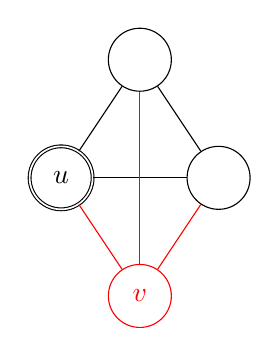
\begin{tikzpicture}
    \node[circle, double, draw, minimum size=8mm] (a) at (0,0) {$u$};
    \node[circle, draw, minimum size=8mm] (b) at (1,1.5) {};
    \node[circle, draw, minimum size=8mm] (c) at (2,0) {};
    \node[circle, draw=red, text=red, minimum size=8mm] (v) at (1,-1.5) {$v$};

    \draw (a) -- (b);
    \draw (a) -- (c);
    \draw (b) -- (c);
    \draw[draw=red] (v) -- (a);
    \draw[draw=red] (v) -- (b);
    \draw[draw=red] (v) -- (c);
\end{tikzpicture}
}

% \inferrule*[Right=SimplicialSingleton]
%     {u \not \in V}
%     {\simplicial{u}{G+u}}
% \\
% \inferrule*[Right=SimplicialNode]
%     {\simplicial{u}{G} \\ u \neq v}
%     {\simplicial{u}{G + v}}
% \\
% \inferrule*[Right=SimplicialEdge]
%     {\simplicial{u}{G} \\ u \neq v' \\ u \neq v''}
%     {\simplicial{u}{G + \{ v', v''\}}}
% \\
% \inferrule*[Right=SimplicialNeighbor]
%     {\simplicial{u}{G}}
%     {\simplicial{u}{\addvertex{G}{N(u)}{v}}}


% \only<1>{
% \[
% \renewcommand{\arraystretch}{1}
% \begin{array}{l}
% B_1 := \text{Block (Normal 1) } [] \ [ \\
% \quad r(0) \leftarrow i(0); \\
% ] \ (\text{jump } B_2) \\
% \\
% B_2 := \text{Block (Normal 2) } [ \\
% \quad r(2) \leftarrow \phi[(0, \ \text{Normal 1}); \ (3, \ \text{Normal 2})] \\
% ] \ [ \\
% \quad r(3) \leftarrow r(2) + 1 \\
% ] \ (\text{if } r(3) < 20 \text{ then } B_2 \text{ else } B_3) \\
% \\
% B_3 := \text{Block (Normal 3) } [] \ [] \ (\text{ret } r(6)) \\
% \end{array}
% \]
% }

% \only<2>{
% \[
% \renewcommand{\arraystretch}{1}
% \begin{array}{l}
% B_1 := \text{Block (Normal 1) } [] \ [ \\
% \quad r(\text{RBX}) \leftarrow i(0); \\
% ] \ (\text{jump } B_2) \\
% \\
% B_2 := \text{Block (Normal 2) } [ \\
% \quad r(\text{RBX}) \leftarrow \phi[(\text{RBX}, \ \text{Normal 1}); \ (\text{RBX}, \ \text{Normal 2})] \\
% ] \ [ \\
% \quad r(\text{RBX}) \leftarrow r(\text{RBX}) + 1 \\
% ] \ (\text{if } r(\text{RBX}) < 20 \text{ then } B_2 \text{ else } B_3) \\
% \\
% B_3 := \text{Block (Normal 3) } [] \ [] \ (\text{ret } r(\text{RBX})) \\
% \end{array}
% \]
% }
\end{frame}

\section{Verification of \texttt{eliminate}}

\begin{frame}{Inductive Definition of the Simplicial Relation}
% Errors

\setlength{\fboxsep}{0pt}

\centering

\trycontr 1
\pause
\trycontr 2

\pause

\trycontr 3
\pause
\trycontr 4
\end{frame}

\begin{frame}{Termination and Partial Correctness of \texttt{eliminate}}
% Errors

\only<1>{
\centering

$\boxed{\simplicial{u}{G}}$ In the context of graph $G$, node $u$ is simplicial.

\vfill

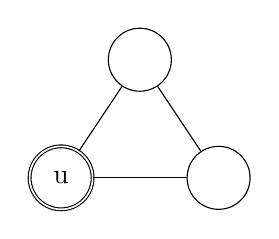
\begin{tikzpicture}
    \node[circle, double, draw, minimum size=8mm] (a) at (0,0) {u};
    \node[circle, draw, minimum size=8mm] (b) at (1,1.5) {};
    \node[circle, draw, minimum size=8mm] (c) at (2,0) {};

    \draw (a) -- (b);
    \draw (a) -- (c);
    \draw (b) -- (c);
\end{tikzpicture}
}

\only<2>{
\[
\inferrule*[Right=SimplicialSingleton]
    {u \not \in V}
    {\simplicial{u}{G+u}}
\]

\vfill

\centering
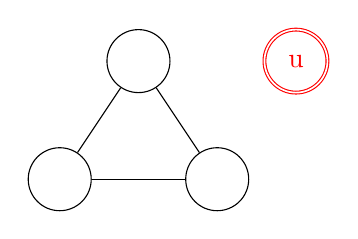
\begin{tikzpicture}
    \node[circle, draw, minimum size=8mm] (a) at (0,0) {};
    \node[circle, draw, minimum size=8mm] (b) at (1,1.5) {};
    \node[circle, draw, minimum size=8mm] (c) at (2,0) {};
    \node[circle, double, draw=red, text=red, minimum size=8mm] at (3,1.5) {u};

    \draw (a) -- (b);
    \draw (a) -- (c);
    \draw (b) -- (c);
\end{tikzpicture}
}

\only<3>{
\[
\inferrule*[Right=SimplicialNode]
    {\simplicial{u}{G}}
    {\simplicial{u}{G + v}}
\]

\vfill

\centering
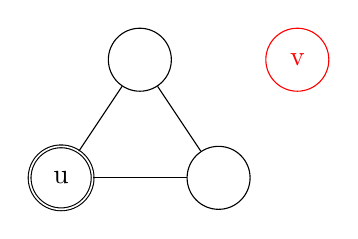
\begin{tikzpicture}
    \node[circle, double, draw, minimum size=8mm] (a) at (0,0) {u};
    \node[circle, draw, minimum size=8mm] (b) at (1,1.5) {};
    \node[circle, draw, minimum size=8mm] (c) at (2,0) {};
    \node[circle, draw=red, text=red, minimum size=8mm] at (3,1.5) {v};

    \draw (a) -- (b);
    \draw (a) -- (c);
    \draw (b) -- (c);
\end{tikzpicture}
}

\only<4>{
\[
\inferrule*[Right=SimplicialEdge]
    {\simplicial{u}{G} \\ u \neq v \\ u \neq w}
    {\simplicial{u}{G + \{ v, w\}}}
\]

\vfill

\centering
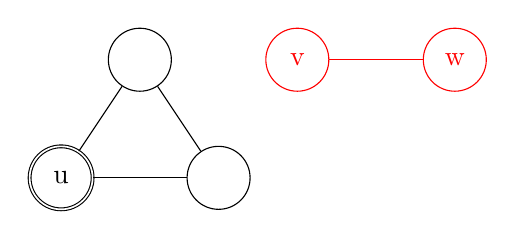
\begin{tikzpicture}
    \node[circle, double, draw, minimum size=8mm] (a) at (0,0) {u};
    \node[circle, draw, minimum size=8mm] (b) at (1,1.5) {};
    \node[circle, draw, minimum size=8mm] (c) at (2,0) {};
    \node[circle, draw=red, text=red, minimum size=8mm] (v) at (3,1.5) {v};
    \node[circle, draw=red, text=red, minimum size=8mm] (w) at (5,1.5) {w};

    \draw (a) -- (b);
    \draw (a) -- (c);
    \draw (b) -- (c);
    \draw[draw=red] (v) -- (w);
\end{tikzpicture}
}

\only<5>{
\[
\inferrule*[Right=SimplicialNeighbor]
    {\simplicial{u}{G}}
    {\simplicial{u}{\addvertex{G}{u}{v}}}
\]

\vfill

\centering
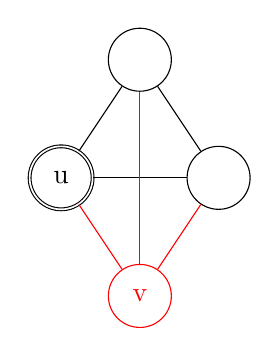
\begin{tikzpicture}
    \node[circle, double, draw, minimum size=8mm] (a) at (0,0) {u};
    \node[circle, draw, minimum size=8mm] (b) at (1,1.5) {};
    \node[circle, draw, minimum size=8mm] (c) at (2,0) {};
    \node[circle, draw=red, text=red, minimum size=8mm] (v) at (1,-1.5) {v};

    \draw (a) -- (b);
    \draw (a) -- (c);
    \draw (b) -- (c);
    \draw[draw=red] (v) -- (a);
    \draw[draw=red] (v) -- (b);
    \draw[draw=red] (v) -- (c);
\end{tikzpicture}
}

% \inferrule*[Right=SimplicialSingleton]
%     {u \not \in V}
%     {\simplicial{u}{G+u}}
% \\
% \inferrule*[Right=SimplicialNode]
%     {\simplicial{u}{G} \\ u \neq v}
%     {\simplicial{u}{G + v}}
% \\
% \inferrule*[Right=SimplicialEdge]
%     {\simplicial{u}{G} \\ u \neq v' \\ u \neq v''}
%     {\simplicial{u}{G + \{ v', v''\}}}
% \\
% \inferrule*[Right=SimplicialNeighbor]
%     {\simplicial{u}{G}}
%     {\simplicial{u}{\addvertex{G}{N(u)}{v}}}


% \only<1>{
% \[
% \renewcommand{\arraystretch}{1}
% \begin{array}{l}
% B_1 := \text{Block (Normal 1) } [] \ [ \\
% \quad r(0) \leftarrow i(0); \\
% ] \ (\text{jump } B_2) \\
% \\
% B_2 := \text{Block (Normal 2) } [ \\
% \quad r(2) \leftarrow \phi[(0, \ \text{Normal 1}); \ (3, \ \text{Normal 2})] \\
% ] \ [ \\
% \quad r(3) \leftarrow r(2) + 1 \\
% ] \ (\text{if } r(3) < 20 \text{ then } B_2 \text{ else } B_3) \\
% \\
% B_3 := \text{Block (Normal 3) } [] \ [] \ (\text{ret } r(6)) \\
% \end{array}
% \]
% }

% \only<2>{
% \[
% \renewcommand{\arraystretch}{1}
% \begin{array}{l}
% B_1 := \text{Block (Normal 1) } [] \ [ \\
% \quad r(\text{RBX}) \leftarrow i(0); \\
% ] \ (\text{jump } B_2) \\
% \\
% B_2 := \text{Block (Normal 2) } [ \\
% \quad r(\text{RBX}) \leftarrow \phi[(\text{RBX}, \ \text{Normal 1}); \ (\text{RBX}, \ \text{Normal 2})] \\
% ] \ [ \\
% \quad r(\text{RBX}) \leftarrow r(\text{RBX}) + 1 \\
% ] \ (\text{if } r(\text{RBX}) < 20 \text{ then } B_2 \text{ else } B_3) \\
% \\
% B_3 := \text{Block (Normal 3) } [] \ [] \ (\text{ret } r(\text{RBX})) \\
% \end{array}
% \]
% }
\end{frame}

\section{Generation of x86-64 Assembly}

\begin{frame}{Generation of x86-64 Assembly}
% Errors



% \inferrule*[Right=SimplicialSingleton]
%     {u \not \in V}
%     {\simplicial{u}{G+u}}
% \\
% \inferrule*[Right=SimplicialNode]
%     {\simplicial{u}{G} \\ u \neq v}
%     {\simplicial{u}{G + v}}
% \\
% \inferrule*[Right=SimplicialEdge]
%     {\simplicial{u}{G} \\ u \neq v' \\ u \neq v''}
%     {\simplicial{u}{G + \{ v', v''\}}}
% \\
% \inferrule*[Right=SimplicialNeighbor]
%     {\simplicial{u}{G}}
%     {\simplicial{u}{\addvertex{G}{N(u)}{v}}}


% \only<1>{
% \[
% \renewcommand{\arraystretch}{1}
% \begin{array}{l}
% B_1 := \text{Block (Normal 1) } [] \ [ \\
% \quad r(0) \leftarrow i(0); \\
% ] \ (\text{jump } B_2) \\
% \\
% B_2 := \text{Block (Normal 2) } [ \\
% \quad r(2) \leftarrow \phi[(0, \ \text{Normal 1}); \ (3, \ \text{Normal 2})] \\
% ] \ [ \\
% \quad r(3) \leftarrow r(2) + 1 \\
% ] \ (\text{if } r(3) < 20 \text{ then } B_2 \text{ else } B_3) \\
% \\
% B_3 := \text{Block (Normal 3) } [] \ [] \ (\text{ret } r(6)) \\
% \end{array}
% \]
% }

% \only<2>{
% \[
% \renewcommand{\arraystretch}{1}
% \begin{array}{l}
% B_1 := \text{Block (Normal 1) } [] \ [ \\
% \quad r(\text{RBX}) \leftarrow i(0); \\
% ] \ (\text{jump } B_2) \\
% \\
% B_2 := \text{Block (Normal 2) } [ \\
% \quad r(\text{RBX}) \leftarrow \phi[(\text{RBX}, \ \text{Normal 1}); \ (\text{RBX}, \ \text{Normal 2})] \\
% ] \ [ \\
% \quad r(\text{RBX}) \leftarrow r(\text{RBX}) + 1 \\
% ] \ (\text{if } r(\text{RBX}) < 20 \text{ then } B_2 \text{ else } B_3) \\
% \\
% B_3 := \text{Block (Normal 3) } [] \ [] \ (\text{ret } r(\text{RBX})) \\
% \end{array}
% \]
% }
\end{frame}

% INDEX
% Title
% Overview
% SLIDE ABOUT RA
% SLIDE ABOUT Graph Coloring RA
% SLIDE ABOUT SSA
% SLIDE ABOUT SSARA
% SLIDE ABOUT JAIR Syntax
% SLIDE ABOUT is_simplicialb
% SLIDE ABOUT find_next
% SLIDE ABOUT eliminate_step

% EXPERIMENTAL INDEX
% Title
% Overview
% SLIDE ABOUT RA
% SLIDE ABOUT Graph Coloring RA
% SLIDE ABOUT SSA
% SLIDE ABOUT SSARA
% SLIDE ABOUT JAIR Syntax
% SLIDE ABOUT is_simplicialb
% SLIDE ABOUT find_next
% SLIDE ABOUT eliminate_step

% %------------------------------------------------
% \section{First Section}
% %------------------------------------------------

% \begin{frame}{Bullet Points}
%     \begin{itemize}
%         \item Lorem ipsum dolor sit amet, consectetur adipiscing elit
%         \item Aliquam blandit faucibus nisi, sit amet dapibus enim tempus eu
%         \item Nulla commodo, erat quis gravida posuere, elit lacus lobortis est, quis porttitor odio mauris at libero
%         \item Nam cursus est eget velit posuere pellentesque
%         \item Vestibulum faucibus velit a augue condimentum quis convallis nulla gravida
%     \end{itemize}
% \end{frame}

% %------------------------------------------------

% \begin{frame}{Blocks of Highlighted Text}
%     In this slide, some important text will be \alert{highlighted} because it's important. Please, don't abuse it.

%     \begin{block}{Block}
%         Sample text
%     \end{block}

%     \begin{alertblock}{Alertblock}
%         Sample text in red box
%     \end{alertblock}

%     \begin{examples}
%         Sample text in green box. The title of the block is ``Examples".
%     \end{examples}
% \end{frame}

% %------------------------------------------------

% \begin{frame}{Multiple Columns}
%     \begin{columns}[c] % The "c" option specifies centered vertical alignment while the "t" option is used for top vertical alignment

%         \column{.45\textwidth} % Left column and width
%         \textbf{Heading}
%         \begin{enumerate}
%             \item Statement
%             \item Explanation
%             \item Example
%         \end{enumerate}

%         \column{.45\textwidth} % Right column and width
%         Lorem ipsum dolor sit amet, consectetur adipiscing elit. Integer lectus nisl, ultricies in feugiat rutrum, porttitor sit amet augue. Aliquam ut tortor mauris. Sed volutpat ante purus, quis accumsan dolor.

%     \end{columns}
% \end{frame}

% %------------------------------------------------
% \section{Second Section}
% %------------------------------------------------

% \begin{frame}{Table}
%     \begin{table}
%         \begin{tabular}{l l l}
%             \toprule
%             \textbf{Treatments} & \textbf{Response 1} & \textbf{Response 2} \\
%             \midrule
%             Treatment 1         & 0.0003262           & 0.562               \\
%             Treatment 2         & 0.0015681           & 0.910               \\
%             Treatment 3         & 0.0009271           & 0.296               \\
%             \bottomrule
%         \end{tabular}
%         \caption{Table caption}
%     \end{table}
% \end{frame}

% %------------------------------------------------

% \begin{frame}{Theorem}
%     \begin{theorem}[Mass--energy equivalence]
%         $E = mc^2$
%     \end{theorem}
% \end{frame}

% %------------------------------------------------

% \begin{frame}{Figure}
%     Uncomment the code on this slide to include your own image from the same directory as the template .TeX file.
%     %\begin{figure}
%     %\includegraphics[width=0.8\linewidth]{test}
%     %\end{figure}
% \end{frame}

% %------------------------------------------------

% \begin{frame}[fragile] % Need to use the fragile option when verbatim is used in the slide
%     \frametitle{Citation}
%     An example of the \verb|\cite| command to cite within the presentation:\\~

%     This statement requires citation \cite{p1}.
% \end{frame}

%------------------------------------------------

% \begin{frame}{References}
%     \footnotesize
%     \bibliography{reference.bib}
%     \bibliographystyle{apalike}
% \end{frame}

%------------------------------------------------

\begin{frame}
    \Huge{\centerline{\textbf{The End}}}
\end{frame}

% %----------------------------------------------------------------------------------------

\end{document}
